\documentclass[fleqn]{jsarticle}

\usepackage{listings,jlisting}
\usepackage[dvipdfmx]{hyperref,graphicx}
\usepackage{ascmac}
\usepackage{color}

\lstset{%
  language={C},
  basicstyle={\small\ttfamily},%
  identifierstyle={\small\ttfamily},%
  commentstyle={\color{magenta}\small\ttfamily\itshape},%
  keywordstyle={\color{blue}\small\bfseries\ttfamily},%
  ndkeywordstyle={\small},%
  stringstyle={\color{red}\small\ttfamily},
  frame={tb},
  breaklines=true,
  columns=[l]{fullflexible},%
  numbers=left,%
  xrightmargin=0zw,%
  xleftmargin=3zw,%
  numberstyle={\scriptsize},%
  stepnumber=1,
  numbersep=1zw,%
  lineskip=-0.5ex,%
  keepspaces=true%
}

\title{サイバーセキュリティ}
\author{
  大阪大学大学院 工学研究科\\
  高野 祐輝
}

\begin{document}

\maketitle

\tableofcontents

% \section{目的と評価方法}

% \begin{quote}
% \begin{description}
%     \item[最優] ファイアウォール技術とペネトレーションテストを組み合わせて,検疫ネットワークの設計と構築を行うことができる
%     \item[優] ファイアウォール技術でDeMilitarized Zoneのあるネットワーク設計と構築を行うことができる
%     \item[良] ファイアウォール技術で適切なネットワークアクセスコントロールができる
%     \item[可] 各種サイバー攻撃手法と防御手法について論じることができる
% \end{description}
% \end{quote}


% \section{セキュリティ哲学}

% \subsection{サイバーセキュリティとは何か}

% \subsection{サイバーキルチェーン}

% \cite{hutchins2011intelligence}

% \subsection{セキュリティポリシとユーザビリティ}

% \cite{RFC2196}

\section{TCP/IPの基礎} \label{sec:tcpip}
\subsection{OSI参照モデル}

インターネットで利用されるプロトコルは、The Internet Engineering Task Force (IETF)という標準化
団体により策定され、その標準はRequest for Comments (RFC)という名のオープンな仕様として発行されている。
例えば、我々が利用しているインターネットプロトコルである
インターネットプロトコル バージョン4は、1981年に791番目のRFCとして策定された~\cite{RFC0791}。

IETF以外の通信に関する標準化団体としては
International Telecommunication Union Telecommunication Standardization Sector (ITU-T)や、
International Organization for Standardization (ISO)が存在する。
実は、1977年から1982年かけて、ITU-TやISOがコンピュータネットワークの標準通信プロトコルとして、
Open Systems Interconnection (OSI)の策定を行っていた。
その当時は標準的な通信プロトコルは存在せず、ベンダーごとに様々なプロトコルが利用されていたため、
通信プロトコルの統一化が求められていたのである。
しかしながら、最終的にOSIは主流とはならず、IETFによって策定された
インターネットプロトコルが広く利用されるようになっていった。

\begin{figure}[tb]
    \centering
    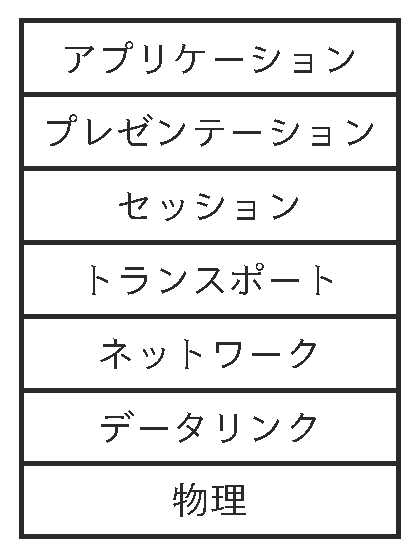
\includegraphics[width=5cm,pagebox=artbox]{figs/OSI.pdf}
    \caption{OSI参照モデル}
    \label{fig:osi}
\end{figure}

OSI自体は残らなかったが、OSI策定の際に考案されたOSI参照モデルと呼ばれる
ネットワークの抽象化手法は、今日でも広く受け入れられている。
図~\ref{fig:osi}は、OSI参照モデルによるネットワークの抽象化モデルを表している。
OSI参照モデルでは、ネットワークの機能を階層構造にもとづいて抽象化しており、
この抽象化をレイヤリングなどと呼ぶ。
OSI参照モデルでは、下から順に1層に物理層、2層にデータリンク層、
3層にネットワーク層、4層にトランスポート層、5層にセッション層、
6層にプレゼンテーション層、7層にアプリケーション層が位置する。
ちなみに、各層のことをレイヤ1、レイヤ2といったり、更に略してL1、L2などということもある。

\begin{figure}[tb]
    \centering
    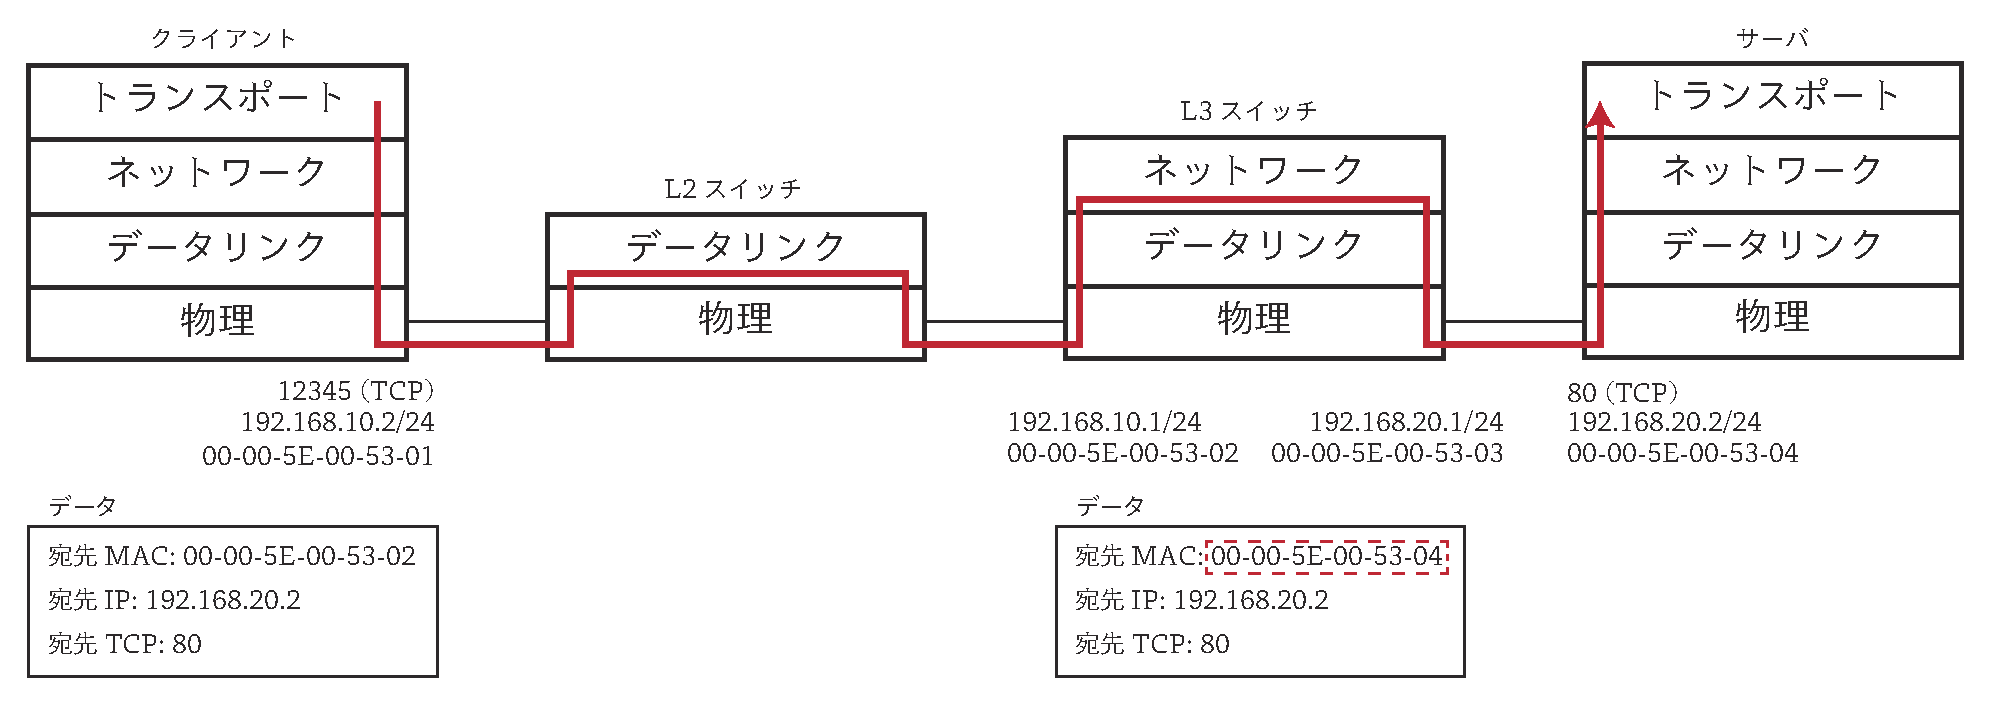
\includegraphics[height=5cm,pagebox=artbox]{figs/osi_link.pdf}
    \caption{各層でのデータ転送}
    \label{fig:osi_link}
\end{figure}

\begin{itembox}[l]{\bf 重要ポイント}
    \begin{itemize}
        \item インターネット関連のプロトコルは、IETFが発行するRFCによって標準化されている
        \item コンピュータネットワークはレイヤで考えることができる
    \end{itemize}
\end{itembox}

\subsection{データリンク層}

\subsection{ネットワーク層}

\subsection{トランスポート層}

\subsection{トランスポートより上の層}

% \section{PF (Packet Filter)の基礎}

\section{演習問題} \label{sec:exercise}

\subsection{ルーティング}


\subsubsection{3ノードの単純なネットワーク}

図~\ref{fig:quiz01}のようなネットワークがあるとする。
このとき、ノードh1からノードh3へ及び、ノードh3からノードh1へIPv4パケットが到達するように、
ノードh1〜h3を設定せよ。(ヒント:ノードh1〜h3のルーティングテーブルをrouteコマンドで設定し、
ノードh2をIPv4のフォワーディングを行うようにsysctlコマンドで設定せよ)

\begin{figure}
    \centering
    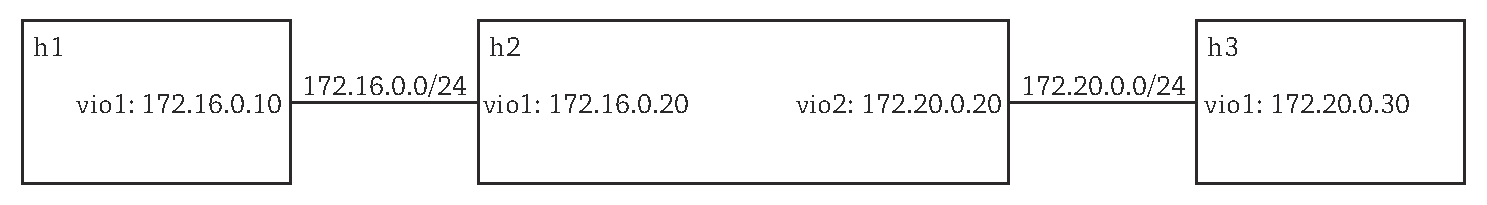
\includegraphics[width=15cm,pagebox=artbox]{figs/quiz01.pdf}
    \caption{問題1:3ノードの単純なネットワークのトポロジ図} \label{fig:quiz01}
\end{figure}

\subsubsection{4ノードのネットワーク}

図~\ref{fig:quiz02}のようなネットワークがあるとする。
このとき、各ノードから全てのノードへIPv4パケットが到達するように、
ノードh1〜h4を設定せよ。

\begin{figure}
    \centering
    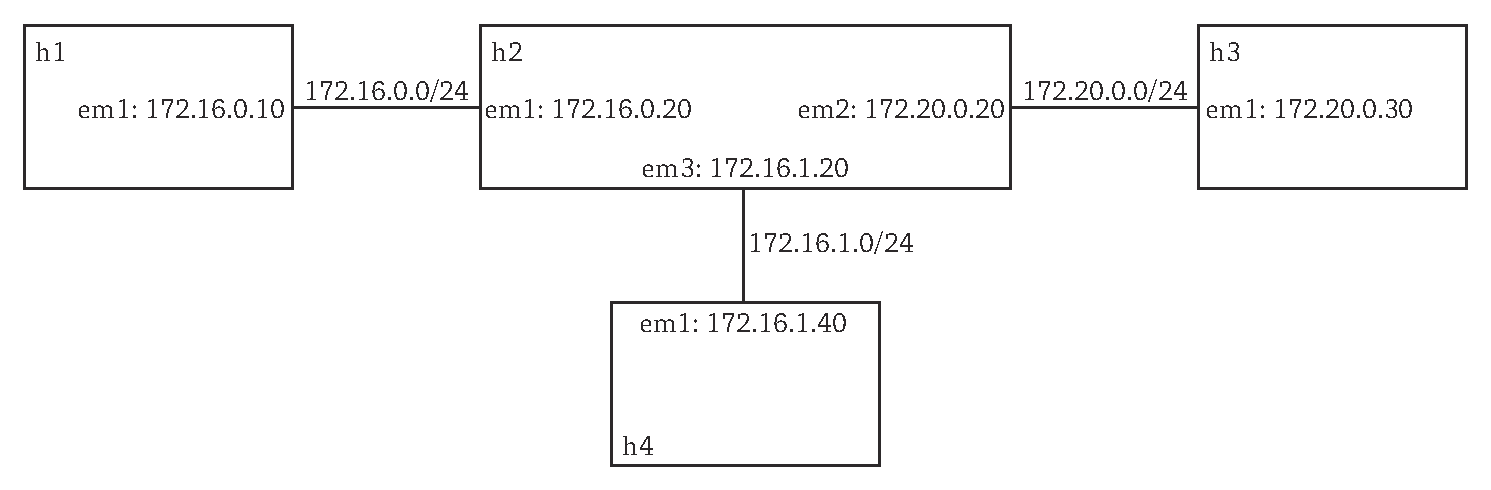
\includegraphics[width=15cm,pagebox=artbox]{figs/quiz02.pdf}
    \caption{問題1:4ノードネットワークのトポロジ図} \label{fig:quiz02}
\end{figure}

\subsection{パケットフィルタ}

\subsubsection{DMZ(DeMilitarized Zone)}


\subsection{VLAN}

\subsection{NAT}

\subsection{ブリッジ}

% \appendix

% \section{Vagrantによる実験環境の構築}

% \section{PFの構文}


\bibliography{ref,rfc} %hoge.bibから拡張子を外した名前
\bibliographystyle{junsrt} %参考文献出力スタイル

\end{document}